\documentclass{article}
%\usepackage{perso}
\RequirePackage{amsmath,amssymb,mathrsfs}
\usepackage{tkz-euclide}
\usepackage[margin=1.5cm]{geometry}
\usetkzobj{all}
\usepackage{enumitem}
\setlist[itemize,1]{label=\textbullet}
%\NewDocumentCommand{\norm}{m}{\lVert#1\rVert}
%\NewDocumentCommand{\norme}{m}{\lVert\V{#1}\rVert}

%\makeatletter
	%\patchcmd{\tkz@DrawLine}{\begingroup}{\begingroup\makeatletter}{}{}
%\makeatother

\begin{document}

\title{Raycasting in cub3d}

\maketitle

\section{The grid}


\begin{center}
  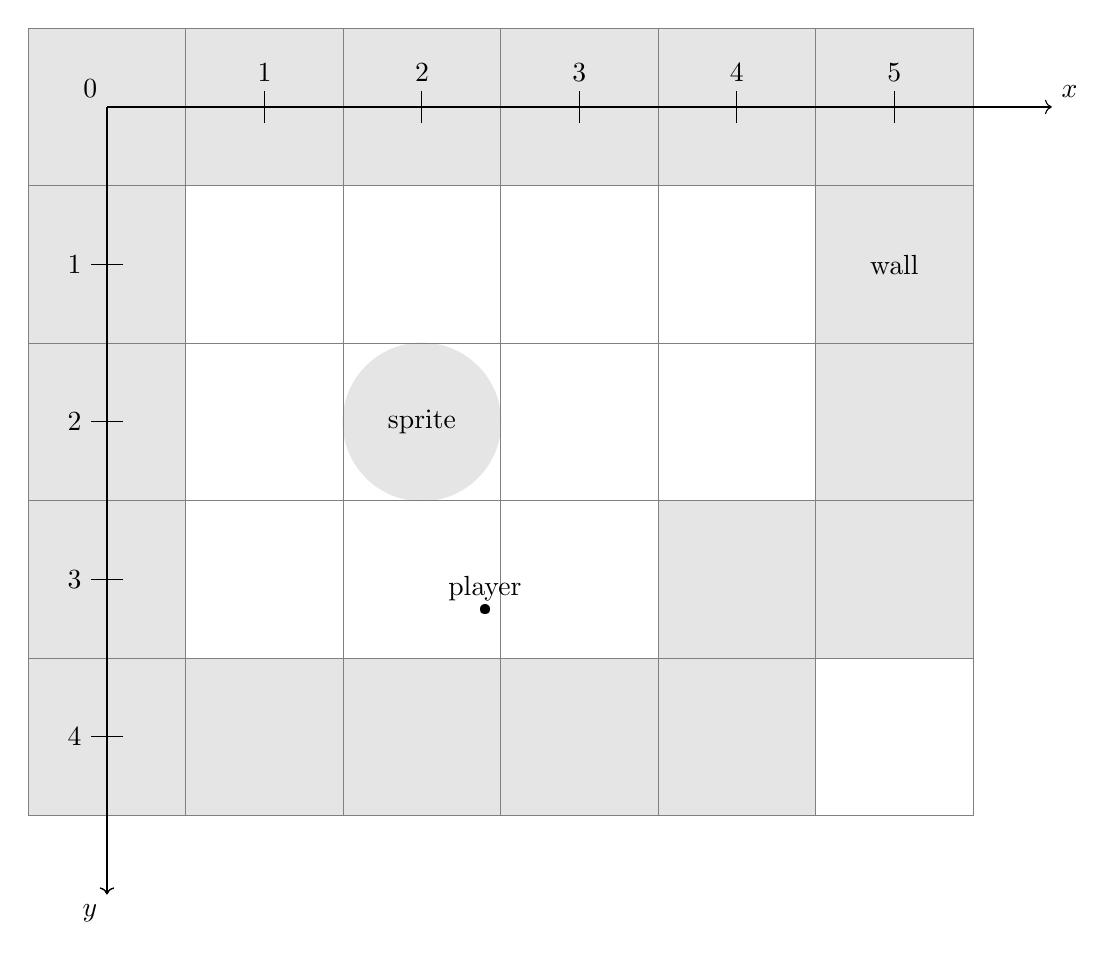
\begin{tikzpicture}[scale=2]
    \draw[fill, gray!20] (-.5,.5)rectangle(.5, -4.5);
    \draw[fill, gray!20] (-.5,-4.5)rectangle(4.5, -3.5);
    \draw[fill, gray!20] (3.5,-3.5)rectangle(4.5, -2.5);
    \draw[fill, gray!20] (4.5,-3.5)rectangle(5.5, .5);
    \draw[fill, gray!20] (-.5,-.5)rectangle(5.5, .5);
    \draw[fill, gray!20] (2,-2)circle(.5);
    \draw (2,-2)node{sprite};
    \draw (5,-1)node{wall};


    \draw[gray] (0,0) grid[xstep=1, ystep=1, xshift=-.5cm, yshift = .5cm](6, -5);
    \draw(0,0)node[above left]{0};
    \foreach \x in {1, ..., 5} \draw(\x, -.1)--(\x,.1)node[above]{\x};
    \foreach \x in {1, ..., 4} \draw(.1, -\x)--(-.1,-\x)node[left]{\x};
    \draw[->](0, 0) -- (0, -5);
    \draw[->](0, 0) -- (0, -5)node[below left]{$y$};
    \draw[->](0, 0) -- (6, 0)node[above right]{$x$};
    \draw (2.4,-3.2)node{\textbullet}node[above]{player};
  \end{tikzpicture}
\end{center}

\newpage
\section{Drawing a pixel column}

\begin{center}
  \begin{tikzpicture}[scale=2]
    \draw (0,0) -- (6,0);
    \draw (0,0) -- (0,4);
    \draw[dashed] (3,0) -- (3,4);

    %Bonhomme
    \draw[fill] (5,2)circle(0.25);
    \draw (5,1) -- (5,1.75);
    \draw (5.25,0) -- (5,1) -- (4.75,0);
    \draw (5.25,1.5) -- (4.75,1.5);

    %Champ de vision
    \draw[dotted] (0,0) -- (5,2);
    \draw[dotted] (0,4) -- (5,2);

    %Distances
    \draw[<->] (2.75,1.2) -- (2.75,2.8)node[midway, left]{perceived\_height};
    \draw[<->] (3.25,0.8) -- (3.25,3.2)node[above right]{screen\_height};
    \draw [<->] (0, -0.75) -- (5, -0.75)node[midway, below]{dist\_to\_wall};
    \draw [<->] (3, -0.25) -- (5, -0.25)node[midway, below]{SCREEN\_DISTANCE};
    \draw [<->] (-0.25, 0) -- (-0.25, 4)node[midway, left]{WALL\_HEIGHT};
    \draw [<->] (6.25, 0) -- (6.25, 2)node[midway, right]{WALL\_HEIGHT / 2};
  \end{tikzpicture}
\end{center}

Hence, we have:

$$\frac{\text{perceived\_height}}{\text{WALL\_HEIGHT}} = \frac{\text{SCREEN\_DISTANCE}}{\text{dist\_to\_wall}}$$

$$\text{perceived\_height} = \text{WALL\_HEIGHT}\times\frac{\text{SCREEN\_DISTANCE}}{\text{dist\_to\_wall}}$$

\newpage

\begin{center}
  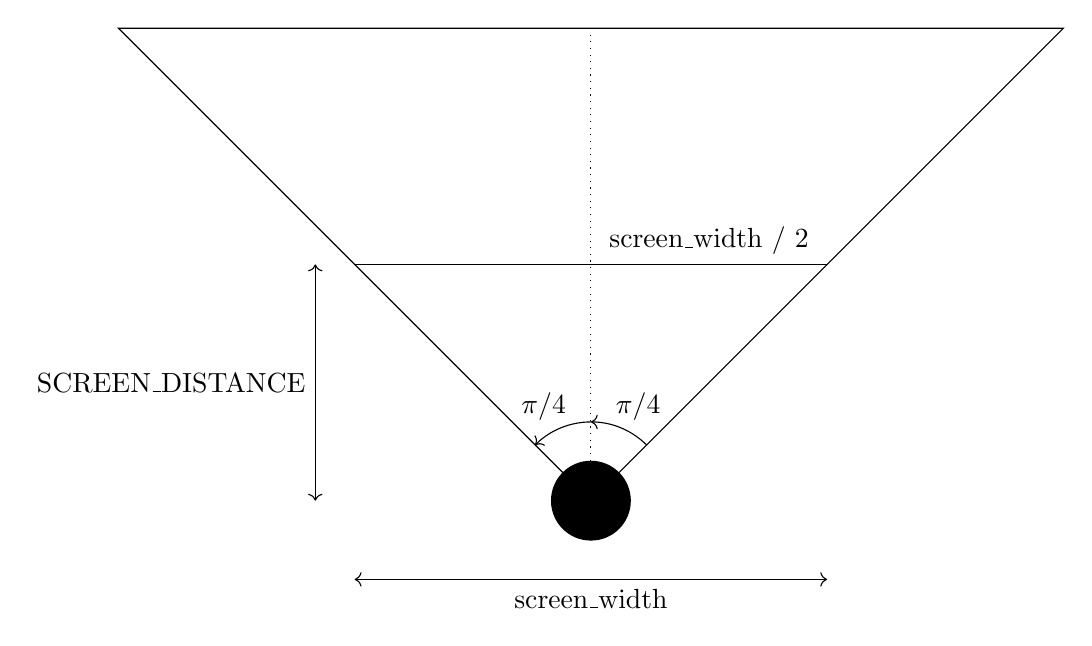
\begin{tikzpicture}[scale=2]
    \coordinate (O) at (0,0);
    \coordinate (B) at (-3,3);
    \coordinate (C) at (3, 3);
    \coordinate (D) at (0, 1.5);

    \draw[fill] (O)circle (0.25);
    \draw (O) -- (B) -- (C) -- cycle;

    \draw[<->] (-1.75,0) -- (-1.75, 1.5)node[midway, left]{SCREEN\_DISTANCE};
    %\draw (-1.5,1.5) -- (0,1.5)node[midway, above]{screen\_width / 2};
    \draw (-1.5,1.5) -- (D) -- (1.5,1.5)node[midway, above]{screen\_width / 2};
    \draw[<->] (-1.5,-0.5) -- (1.5,-0.5)node[midway, below]{screen\_width};


    \tkzMarkAngle[arrows=->, size=0.5](C,O,D)
    \tkzMarkAngle[arrows=->, size=0.5](D,O,B)
    \draw (.3,.6)node{$\pi / 4$};
    \draw (-.3,.6)node{$\pi / 4$};
    \draw[dotted] (O) -- (0, 3);
  \end{tikzpicture}
\end{center}

Hence:

$$\tan\left(\frac\pi4\right) = \frac{\text{screen\_width} / 2}{\text{SCREEN\_DISTANCE}}$$

$$1 = \frac{\text{screen\_width}}{2\times\text{SCREEN\_DISTANCE}}$$

$$\text{screen\_width} = 2\times\text{SCREEN\_DISTANCE}$$

\vspace{2cm}

\begin{center}
  \begin{tikzpicture}[scale=1]
    \coordinate (A) at (0,0);
    \coordinate (B) at (0,3);
    \coordinate (C) at (5,2);
    \coordinate (D) at (5,5);

    \draw (A) -- (B)node[midway, left]{screen\_height} -- (D)  node[midway, yshift = .6cm]{screen\_width} -- (C) -- cycle;
  \end{tikzpicture}
\end{center}

If $(\text{res.x}, \text{res.y})$ is the resolution of the window:

$$\frac{\text{screen\_height}}{\text{res.y}} = \frac{\text{screen\_width}}{\text{res.x}}$$

$$\text{screen\_height} = \text{res.y}\times\frac{\text{screen\_width}}{\text{res.x}}$$

As showed above, $\text{screen\_width} = 2\times\text{SCREEN\_DISTANCE}$, so


$$\text{screen\_height} = 2\times\text{SCREEN\_DISTANCE} \times \text{res.y} \div \text{res.x}$$


\newpage

\section{Drawing a sprite}

\begin{center}
  \begin{tikzpicture}[scale=1]
    \coordinate (C) at (6,6);
    \coordinate (P) at (0,0);
    \coordinate (K) at (6,0);

    \draw (P)node[below]{$P$} -- (C)node[right]{$C$} circle(1);
    \draw (P) -- (7,0);
    \draw (P) -- (K)node[midway, below]{$x_C - x_P$};

    \draw[dotted] (C) -- (K)node[midway, right]{$y_C - y_P$};
    
    \tkzMarkAngle[size=1.5, arrows=->](K,P,C)
    \draw (1.8,0.5)node{$\alpha$};

    \draw (C) ++ (-0.71,0.71) -- (C);
    \draw (C) ++ (-0.71,0.71) -- (P);
    \draw (C) ++ (0.71,-0.71) -- (C);
    \draw (C) ++ (0.71,-0.71) -- (P);

    \draw[<->] (7.5,5)--(7.5,7)node[midway, right]{1};
  \end{tikzpicture}
\end{center}

\def\atan{{\rm atan}}
$$\alpha = \atan\left(\frac{y_C - y_P}{x_C - x_P}\right)$$

\begin{center}
  \begin{tikzpicture}[scale=2]
    \coordinate (P) at (0,0);
    \coordinate (C) at (5,0);
    \coordinate (K) at (5,1);

    \draw(P)node[below]{$P$} -- (5,0)node[midway, below]{dist\_to\_sprite};
    \draw[dashed] (P) -- (5, -1);
    \draw[dashed] (P) -- (5, 1);
    \draw (3.5,.5)node{d'};
    \draw (P) -- (5, -2) -- (5, 2) -- cycle;
    \draw (C)node[right]{$C$};

    \tkzMarkAngle[size=1.5](C,P,K)
    \draw (1.5,0.2)node[right]{$\beta$};

    %Distances
    \draw[<->] (-.5, 0)--(-.5,2)node[midway, left]{0.5};
  \end{tikzpicture}
\end{center}

$$\cos(\beta) = \frac{PC}{d'} = \frac{\text{dist\_to\_sprite}}{d'}$$

$$d' = \frac{\text{dist\_to\_sprite}}{\cos(\beta)}$$

\end{document}
